\SourceLeaf{602}folgende Aufsätze aus. I. Bemerkungen über die Einrichtung magnetischer Observatorien und Beschreibung der darin aufzustellenden Instrumente. Vielen Lesern wird es angenehm sein, dass dabei auch die Kosten und Preise angegeben sind. II. Das in den Beobachtungsterminen anzuwendende Verfahren. III. Auszug aus dreijährigen Beobachtungen der magnetischen Declination zu Göttingen. IV. Beschreibung eines kleinen Apparats für Reisende zur Messung der Intensität des Erdmagnetismus nach absolutem Maasse. V. Erläuterungen zu den (hier gelieferten) Terminszeichnungen und den Beobachtungszahlen.

Die übrigen vier Steindrucktafeln geben einen Situationsplan des Göttingischen magnetischen Observatoriums: eine perspectivische Darstellung des Beobachtungssaales und der darin aufgestellten Instrumente, den Grundriss desselben, und genaue Abbildungen aller einzelnen Theile des Magnetometers.

\Needspace{20\baselineskip}\vspace{6mm}
\pdfbookmark[1]{Die neue Einrichtung des Marburger mathematisch-physikalischen Instituts.}{gerling-institut-1842}
\begin{center}\small Göttingische gelehrte Anzeigen.\quad 1842.\quad April 4.\end{center}

Herr Prof.\ \textsc{Gerling} in Marburg, Correspondent der königl.\ Societät, hat in einem Schreiben an Herrn Hofr.\ \textsc{Gauss} einen Bericht über
\begin{center}\textit{die neue Einrichtung des dortigen mathematisch-physikalischen Instituts}\end{center}
mitgetheilt, woraus wir hier einen Auszug um so lieber geben, da bei jener nicht blos auf die gewöhnlichen Bedürfnisse des Unterrichts, sondern auch auf die Wissenschaft selbst Bedacht genommen ist, und die Localität mehrere Eigenthümlichkeiten darbietet.

Das Institut hat seit vorigem Herbst sein Local in einem auf Befehl seiner Hoheit des Kurprinzen und Mitregenten umgebauten und der Universität überwiesenen Staatsgebäude, dem so genannten Dörnberger Hofe. Das zweite Stockwerk enthält ausser dem Auditorium vier helle Säle, ein kleineres Zimmer, welches zu optischen Versuchen verdunkelt werden kann, und noch zwei besondere Arbeitszimmer. Durch die so geräumige Aufstellung der Instrumente ist bezweckt, dass jedes einzelne Instrument an seinem Platze unmittelbar benutzt werden kann, ohne dass dadurch der gleichzeitige Gebrauch anderer verhindert oder
\SourceLeaf{603}gestört wird, und dass eigene Übungen solcher Studirenden, die dazu Neigung und hinlängliche Vorbereitung haben, mit Bequemlichkeit geschehen können. Das Institut besitzt übrigens schon einen reichen physikalischen Apparat, der jährlich noch vervollständigt und vermehrt wird. Bei geöffneten Zwischenthüren bietet diese Reihe von Zimmern eine freie gerade Linie von 150 Fuss Länge dar, ein für mancherlei Zwecke in der That sehr schätzbarer Vortheil.

Die Officialwohnung des Directors befindet sich im dritten Stockwerk; auch hat das Institut eine eigene Werkstatt und Schmiede, die in das Erdgeschoss verlegt sind.

Zu Versuchen, die im Freien angestellt werden müssen, findet sich hinlängliche Gelegenheit sowohl in der Umgebung des Gebäudes, als auf der Plattform eines mit diesem in unmittelbarer Verbindung stehenden auf dem Felsen gegründeten Thurms. Dieser bietet zugleich ein bei manchen physikalischen Arbeiten überaus schätzbares Hülfsmittel dar, nemlich eine freie Fallhöhe von etwa 80 Fuss. Um diese zu erlangen, sind die Fussböden in den drei Stockwerken des Thurms so wie über dem Keller (ehemaligem Verlies) mit quadratischen Öffnungen durchbrochen; zugleich befindet sich auf der obern Plattform, zu welcher vom Hausdache aus eine Wendeltreppe führt, ein achteckiger Pavillon von 15 Fuss Durchmesser, in dessen Fussboden eine ähnliche Öffnung ist. die je nach Umständen mit einer Fallthür zugelegt, oder mit einer Gallerie umgeben werden kann. In dem Thurme findet sich auch eine nahe 20 Fuss hohe, sehr feste Mauer, die bei manchen Gelegenheiten wichtige Vortheile gewähren kann.

In Verbindung mit dieser Einrichtung wurde nun auch Abhülfe für ein Bedürfniss gewonnen, welches an einer Universität, die keine Sternwarte besitzt, und wo also z.\ B.\ die zu so vielen physikalischen Geschäften jetzt unentbehrlichen Zeitbestimmungen bisher immer blos durch Zeit raubende correspondirende Sonnenhöhen erhalten werden konnten, besonders fühlbar wird. Es war dazu nur nöthig, den Thüren und Fenstern jenes Pavillons eine angemessene Einrichtung zu geben, um denselben zu allen erforderlichen Beobachtungen mit den beweglichen astronomischen Instrumenten brauchbar zu machen, welche das Institut zum Theil schon lange besass. Ein \textsc{Ertel}sches tragbares Passageninstrument z.\ B.\ hat von seinem regelmässigen Standpunkte aus einen ganz freien Spielraum, im Meridian von Horizont zu Horizont, und im ersten Vertical vom westlichen Horizont bis zu etwa 11 Grad östlicher Zenithdistanz. Die Lage dieses Platzes
\SourceLeaf{604}ist durch die von Herrn Prof.\ \textsc{Gerling} ausgeführte, an die hannoversche Gradmessung angeknüpfte trigonometrische Vermessung des Kurfürstenthums, deren ausführlicher Bekanntmachung wir mit Verlangen entgegensehen, gefunden: Breite $50^0\;48'\;46''9$, Länge von Ferro $26^0\;26'\;2''3$.

Endlich muss noch einer Einrichtung Erwähnung geschehen, welche als wesentlich zur Vollendung des ganzen Planes betrachtet wurde. So ganz vorzüglich sich auch das Hauptgebäude für alle übrigen Zwecke eignete, so hatte es doch den Mangel, dass es verhältnissmässig am wenigsten zu meteorologischen Beobachtungen sich benutzen liess, da es von dem bedeutend höhern Schlossberge überragt wird. Ausserdem bleibt es für mancherlei Zwecke sehr wünschenswerth, zwei ziemlich weit von einander getrennte und doch gegenseitig erreichbare Locale bereit zu haben. Diesem zweifachen Bedürfnisse wurde dadurch abgeholfen, dass ein vorhandenes altes Thürmchen auf dem höchsten Punkte des Schlossberges, in gerader Linie 1900 Fuss entfernt und etwa 100 Fuss höher liegend, zu einem meteorologischen Thurm ausgebaut wurde. Hiedurch ist mithin unter andern vermittelt, dass entfernt von der Stadt, und also mit Beseitigung jeder denkbaren Gefahr, ein Blitzableiter zu Beobachtungen vorgerichtet werden kann, und auch die Möglichkeit gegeben ist, demnächst z.\ B.\ Versuche, die sich auf magnetische Telegraphie beziehen, hier anzustellen.

\clearpage
\SourceLeaf{605}\pdfbookmark[0]{Handschriftlicher Nachlass.}{handschriftlicher-nachlass}
\thispagestyle{empty}
\vspace*{35mm}
\begin{center}
{\large HANDSCHRIFTLICHER}\par\vspace{20mm}
{\LARGE NACHLASS.}
\end{center}
\clearpage
\SourceLeaf{607}\fancyhead[L]{\small HANDSCHRIFTLICHER NACHLASS.}
\pdfbookmark[1]{Zur mathematischen Theorie der electrodynamischen Wirkungen.}{electrodynamische-wirkungen}
\begin{center}
{\large ZUR MATHEMATISCHEN THEORIE}\par\vspace{3mm}
{\large DER ELECTRODYNAMISCHEN WIRKUNGEN.}
\end{center}
\begin{center}[1.]\end{center}
Das allgemeine Grundgesetz für die \textit{Intensität in den einzelnen Theilen eines galvanischen Stromsystems} wird sich auf folgende Ansicht zurückführen lassen:

Man hat nur nöthig, Drähte von gleicher Dicke in Betracht zu ziehen, da man für ungleichförmige durch die Zahl der Drähte aushelfen kann; wäre z.\ B.\ ein Draht in einem Theile $=2$, in einem andern $=3$ stark, so könnte man dafür das System
\begin{center}\resizebox{.62\linewidth}{!}{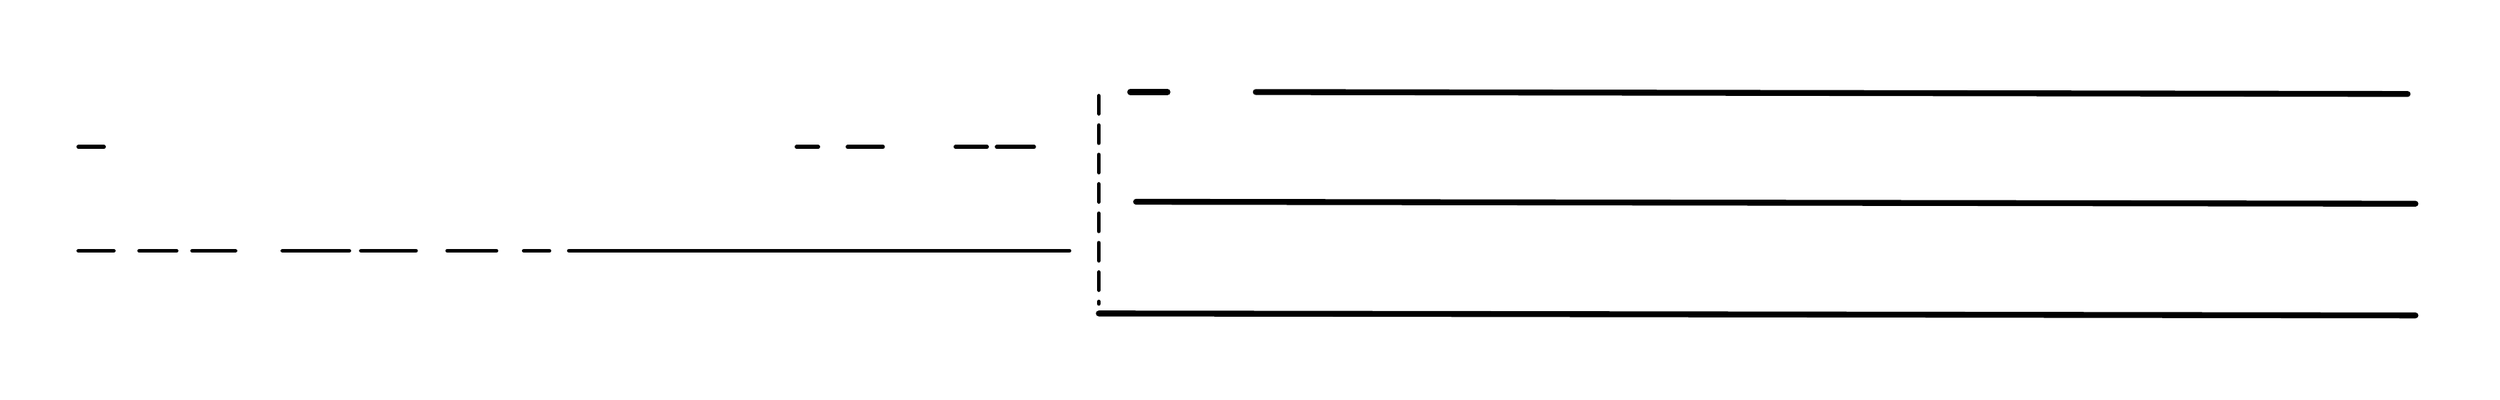
\begin{tikzpicture}[x=1bp,y=-1bp,line cap=round,line join=round]
\path[use as bounding box] (0,0) rectangle (1254,184);
\begin{pgfinterruptboundingbox}
\draw[line width=2bp] (30,65) -- (43,65);
\draw[line width=2bp] (396,65) -- (407,65);
\draw[line width=2bp] (422,65) -- (440,65);
\draw[line width=2bp] (477,65) -- (493,65);
\draw[line width=2bp] (498,65) -- (517,65);
\draw[line width=2bp] (30,118) -- (48,118);
\draw[line width=2bp] (61,118) -- (80,118);
\draw[line width=2bp] (88,118) -- (110,118);
\draw[line width=2bp] (134,118) -- (168,118);
\draw[line width=2bp] (174,118) -- (202,118);
\draw[line width=2bp] (218,118) -- (243,118);
\draw[line width=2bp] (257,118) -- (270,118);
\draw[line width=2bp] (280,118) -- (535,118);
\draw[line width=3bp] (566,37) -- (585,37);
\draw[line width=3bp] (630,37) -- (1217,38);
\draw[line width=3bp] (569,93) -- (1221,94);
\draw[line width=3bp] (550,150) -- (1221,151);
\draw[line width=2.1bp,dash pattern=on 9bp off 6bp] (550,39) -- (550,145);
\end{pgfinterruptboundingbox}
\end{tikzpicture}
}\end{center}
substituiren.

So handelt es sich um die Intensität an jeder Stelle eines zu einem Netz verknüpften Systems von Linien
\begin{center}\resizebox{.63\linewidth}{!}{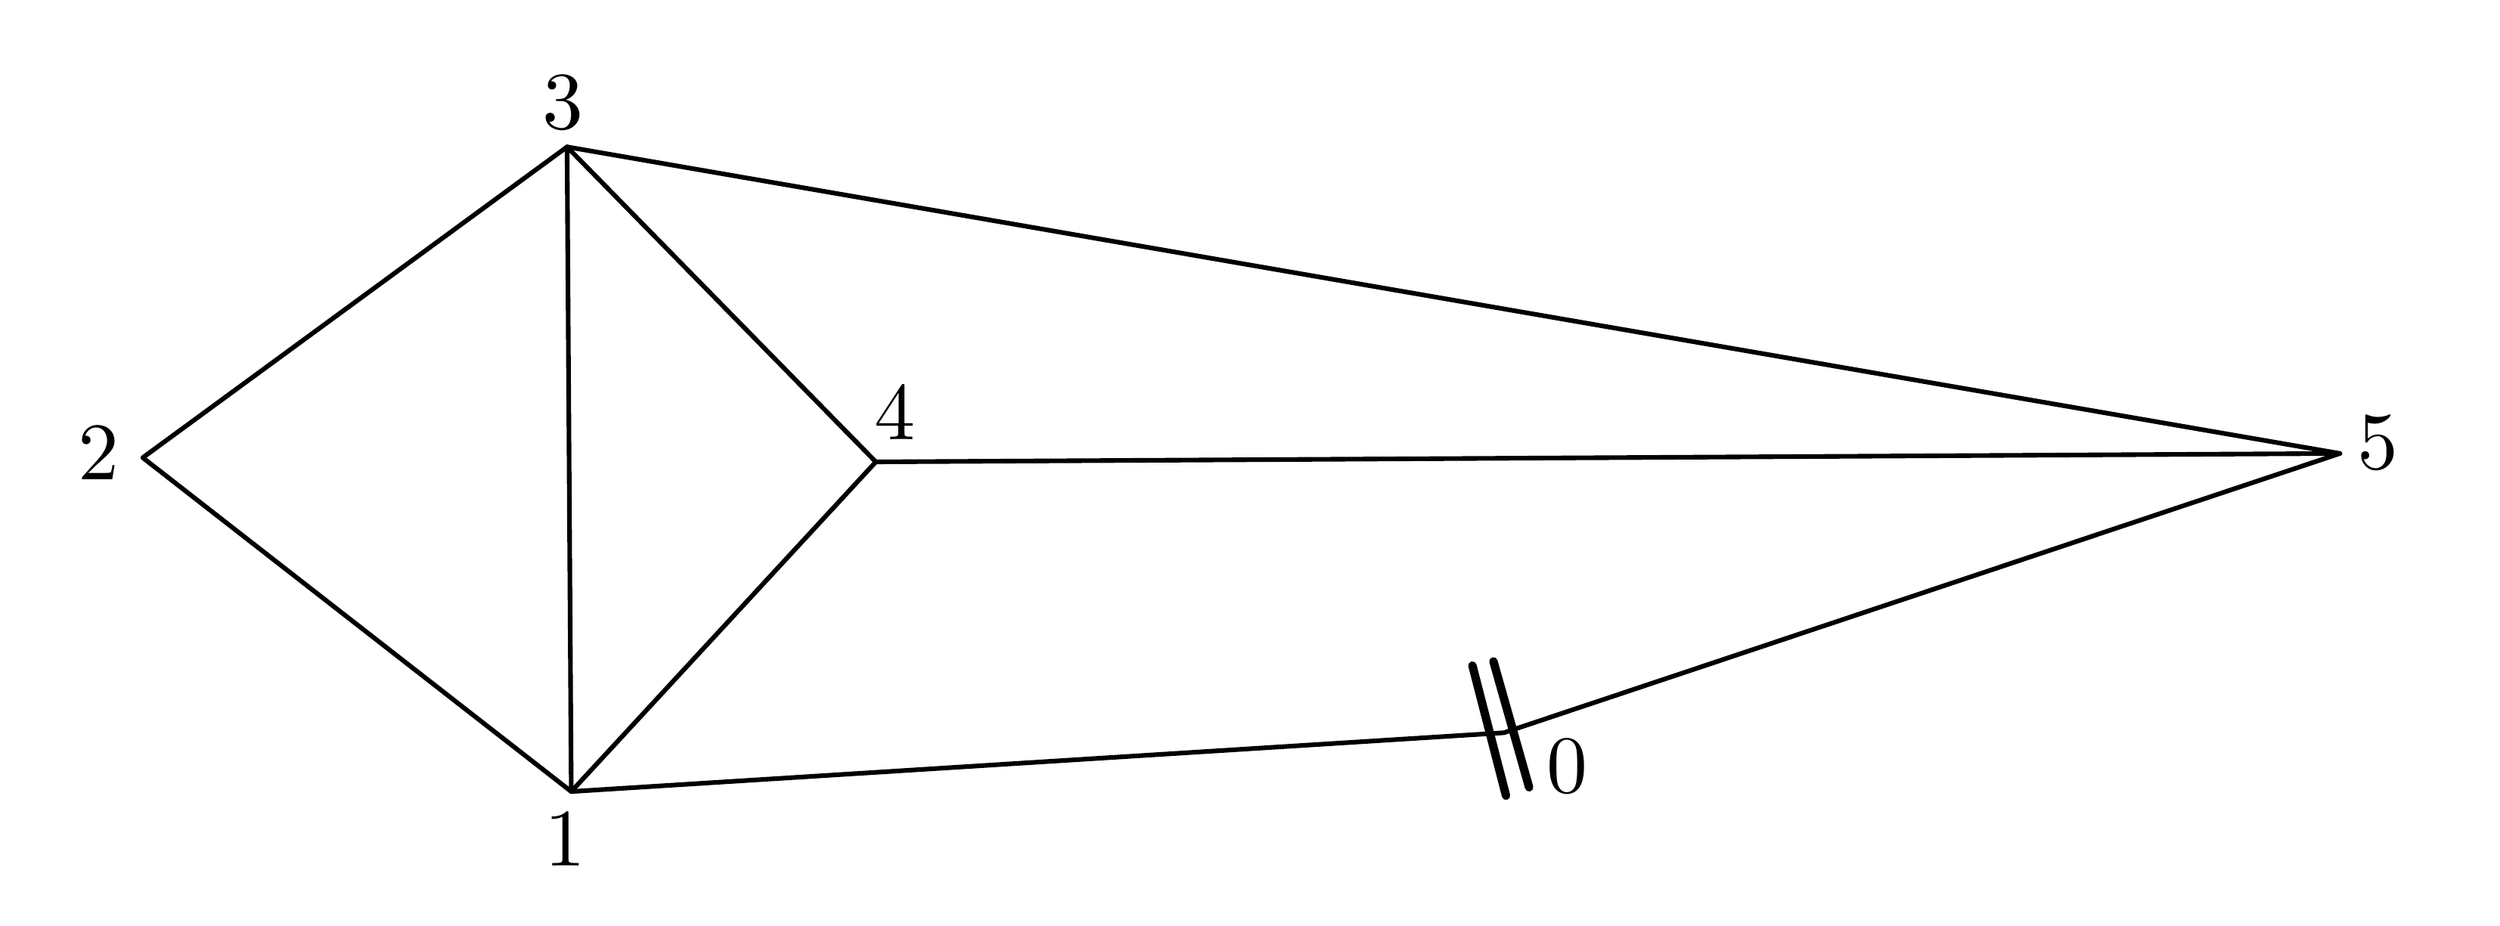
\begin{tikzpicture}[x=1bp,y=-1bp,line cap=round,line join=round]
\path[use as bounding box] (0,0) rectangle (1170,421);
\begin{pgfinterruptboundingbox}
\draw[line width=2.2bp] (262,367) -- (58,208) -- (260,60) -- (407,210) -- (262,367);
\draw[line width=2.2bp] (260,60) -- (262,367);
\draw[line width=2.2bp] (260,60) -- (1104,206) -- (407,210);
\draw[line width=2.2bp] (262,367) -- (706,339) -- (1104,206);
\draw[line width=4bp] (691,307) -- (707,369);
\draw[line width=4bp] (701,305) -- (718,365);
\node[inner sep=0pt,outer sep=0pt] at (259,390) {\scalebox{3.9}{\ensuremath{1}}};
\node[inner sep=0pt,outer sep=0pt] at (37,206) {\scalebox{3.9}{\ensuremath{2}}};
\node[inner sep=0pt,outer sep=0pt] at (258,39) {\scalebox{3.9}{\ensuremath{3}}};
\node[inner sep=0pt,outer sep=0pt] at (416,187) {\scalebox{3.9}{\ensuremath{4}}};
\node[inner sep=0pt,outer sep=0pt] at (1122,201) {\scalebox{3.9}{\ensuremath{5}}};
\node[inner sep=0pt,outer sep=0pt] at (736,355) {\scalebox{3.9}{\ensuremath{0}}};
\end{pgfinterruptboundingbox}
\end{tikzpicture}
}\end{center}
Man braucht statt derselben nur die Punkte, wo mehr als 2 Linien zusammentreffen, und die Kraftsitze zu betrachten. Für jeden Punkt des Systems hat die Intensität \textit{einen} Werth, für die Kraftsitze \textit{zwei}.

\SourceLeaf{608}Das allgemeine Grundgesetz ist nun, dass wenn $A$ ein beliebiger Punkt ist, $A',\ A'',\ A'''\,.\,.$ Punkte, die jeder mit $A$ einfach verbunden sind, und es keinen Punkt $B$ gibt, so dass nicht $AB$ entweder ein Stück von $AA',\ AA'',\ AA'''\,.\,.$ wäre oder umgekehrt, man für jeden Punkt etwas einer Höhe analoges anzunehmen hat, also $a$ im Punkt $A$; $a'$ im Punkt $A'$ u.\ s.\ w., dass dann immer
\[
0=\frac{a'-a}{AA'}+\frac{a''-a}{AA''}+\frac{a'''-a}{AA'''}+\,.\,.
\]
und dass dann immer die einzelnen Theile dieses Aggregats die Stromintensität in den einzelnen Theilen ausdrücken.

\vspace{3mm}
Die allgemeine Auflösung obiger Aufgabe besteht in Folgendem: Es seien $A^0,\ A^{n+1}$ die beiden Pole, $A',\ A'',\ A'''$ etc.\ $A^n$ die einzelnen Knotenpunkte des Systems, $\frac{1}{f^{\alpha,\beta}}$ der ganze Widerstand auf dem einfachen Wege von $A^\alpha$ nach $A^\beta$, wo also der Nenner $=0$ zu setzen ist, wenn zwischen den Punkten eine directe Verbindung fehlt; man bestimme aus den Gleichungen
\[
\begin{aligned}
(f^{1,0}+f^{1,2}+f^{1,3}+\,.\,.)p'-f^{1,0}p^0-f^{1,2}p''-f^{1,3}p'''-\text{etc.}&=0\\
(f^{2,0}+f^{2,1}+f^{2,3}+\,.\,.)p''-f^{2,0}p^0-f^{2,1}p'-f^{2,3}p'''-\text{etc.}&=0\\
(f^{3,0}+f^{3,1}+f^{3,2}+\,.\,.)p'''-f^{3,0}p^0-f^{3,1}p'-f^{3,2}p''-\text{etc.}&=0
\end{aligned}
\]
u.\ s.\ w.\quad in Verbindung mit folgenden
\[
p^0\ \text{willkürlich},\quad p^{n+1}=p^0+k,\quad k\ \text{die erzeugende Kraft bedeutend},
\]
die Grössen $p',p'',p'''\,.\,.$ dann ist Stromkraft zwischen $A^\alpha$ und $A^\beta$
\[
=f^{\alpha,\beta}(p^\beta-p^\alpha)
\]

\vspace{3mm}
Noch einfacher lässt sich das Grundprincip folgendermaassen darstellen.

In jedem Punkt findet ein \textit{bestimmter} Druck statt, sobald an \textit{Einem} Punkt dessen Werth willkürlich angenommen ist. Zwei Sätze reichen dann zu, alles in Gleichungen zu bringen.

I.\quad Sind $A,\ B$ zwei Punkte, zwischen welchen kein Knotenpunkt ist, ist $P$ die Summe der Kräfte zwischen diesen Punkten von $A$ nach $B$ zugeschätzt, $\rho$ der Gesammtwiderstand zwischen diesen Punkten; $a,\ b$ die Werthe des Drucks für jene Punkte, so ist $\frac{a-b+P}{\rho}=$ Intensität des Stromes von $A$ nach $B$ zu.

\SourceLeaf{609}II.\quad Die Summe der Intensitäten aller Ströme von Einem Punkte aus gerechnet (mehr als zwei wenn ein Knotenpunkt) ist $=0$.

\begin{center}[2.]\end{center}
In dem Schema, seien $a,b,c,d,e,f$ die Widerstände in den bezeichneten Stücken, in $a$ die Stromquelle, ferner
\begin{center}\resizebox{.28\linewidth}{!}{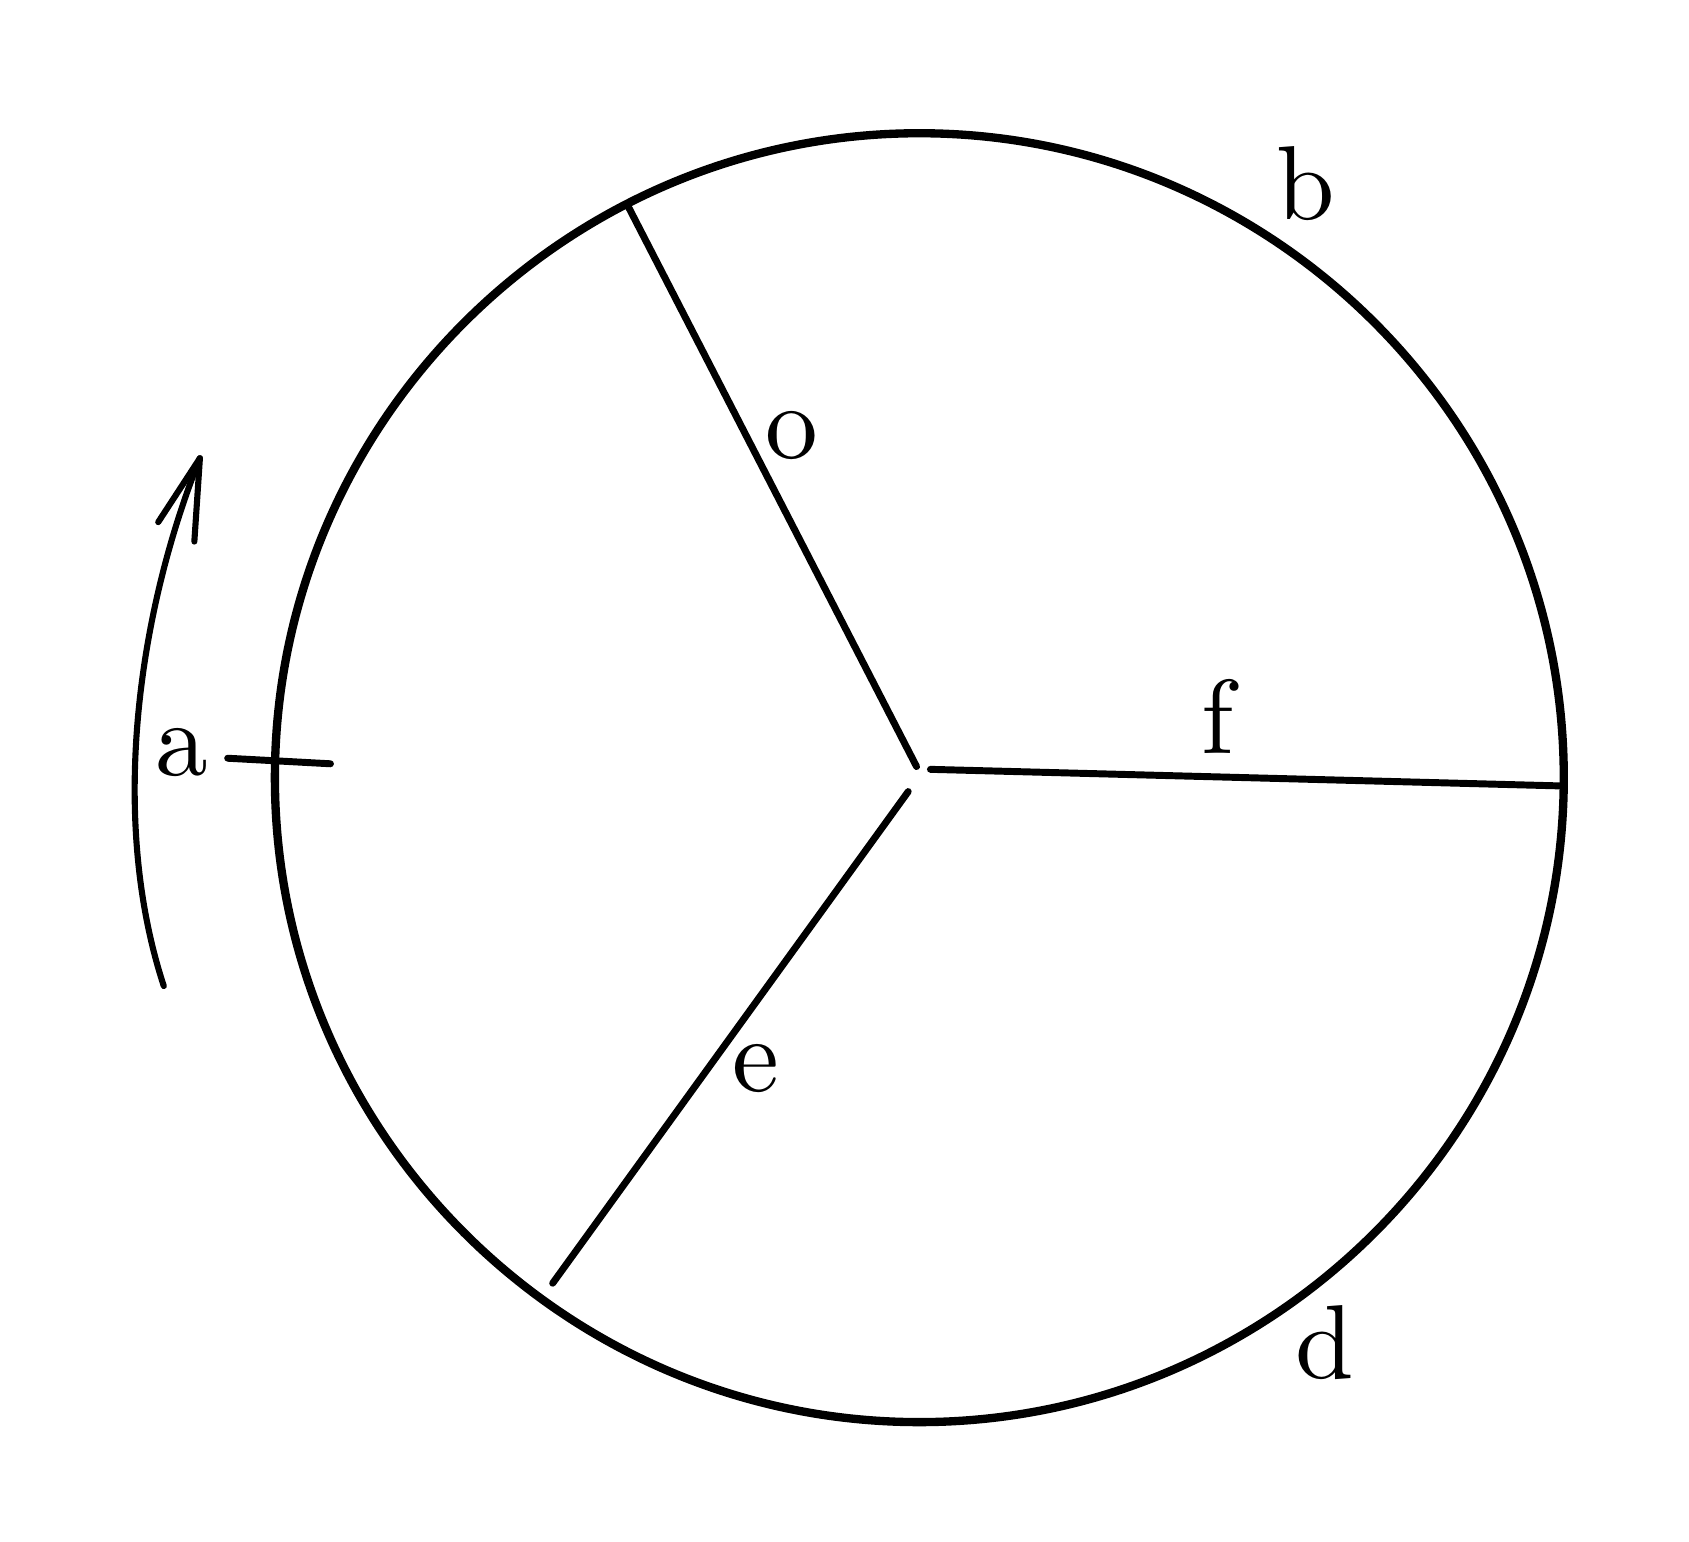
\begin{tikzpicture}[x=1bp,y=-1bp,line cap=round,line join=round]
\path[use as bounding box] (0,0) rectangle (588,535);
\begin{pgfinterruptboundingbox}
\draw[line width=3bp] (321,38) .. controls (448.60,38) and (553,142.40) .. (553,270) .. controls (553,397.60) and (448.60,502) .. (321,502) .. controls (193.40,502) and (89,397.60) .. (89,270) .. controls (89,142.40) and (193.40,38) .. (321,38);
\draw[line width=2.5bp] (216,64) -- (320,266);
\draw[line width=2.5bp] (325,267) -- (553,273);
\draw[line width=2.5bp] (317,275) -- (189,452);
\draw[line width=2.5bp] (72,263) -- (109,265);
\draw[line width=2.2bp] (49,345) .. controls (29,284) and (40,210) .. (62,155);
\draw[line width=2.2bp] (47,178) -- (62,155) -- (60,185);
\node[inner sep=0pt,outer sep=0pt] at (55,261) {\scalebox{3.8}{\ensuremath{\mathrm{a}}}};
\node[inner sep=0pt,outer sep=0pt] at (460,56) {\scalebox{3.8}{\ensuremath{\mathrm{b}}}};
\node[inner sep=0pt,outer sep=0pt] at (275,147) {\scalebox{3.8}{\ensuremath{\mathrm{o}}}};
\node[inner sep=0pt,outer sep=0pt] at (467,473) {\scalebox{3.8}{\ensuremath{\mathrm{d}}}};
\node[inner sep=0pt,outer sep=0pt] at (262,375) {\scalebox{3.8}{\ensuremath{\mathrm{e}}}};
\node[inner sep=0pt,outer sep=0pt] at (430,248) {\scalebox{3.8}{\ensuremath{\mathrm{f}}}};
\end{pgfinterruptboundingbox}
\end{tikzpicture}
}\end{center}
\[
\begin{aligned}
(b+c)(d+e)+f(b+d+c+e)&=p\\
bcde\left(\frac{1}{b}+\frac{1}{c}+\frac{1}{d}+\frac{1}{e}\right)+f(b+d)(c+e)&=q
\end{aligned}
\]
dann ist der Gesammtwiderstand des Systems ohne das Stück $a$
\[
=\frac{q}{p}
\]
die Intensität
\[
\begin{aligned}
A&=\frac{(b+c)(d+e)+f(b+c+d+e)}{ap+q}=\frac{p}{ap+q}\\[4pt]
B&=\frac{cd+ce+cf+ef}{ap+q}\\[4pt]
C&=\frac{bd+be+bf+df}{ap+q}\\[4pt]
D&=\frac{be+ce+cf+ef}{ap+q}\\[4pt]
E&=\frac{bd+cd+bf+df}{ap+q}\\[4pt]
F&=\frac{be-cd}{ap+q}
\end{aligned}
\]
Das Grundprincip führt zugleich dahin, dass
\[
\sum rii
\]
ein Minimum sein muss, wo $r$ den einem Elemente entsprechenden Widerstand, $i$ die Intensität des Stromes bedeuten. Noch einfacher muss
\[
\sum\varepsilon vv
\]
ein Minimum werden, wo $\varepsilon$ ein Element des bewegten Fluidum, $v$ die Geschwindigkeit bedeutet.

\SourceLeaf{610}Sind in einem Leitungsnetz 0, 1, 2 etc.\ die Knotenpunkte
\begin{center}\begin{tabular}{rl}
$r^{01}$ & der Widerstand\\
$i^{01}$ & die Stromstärke von 0 nach 1\\
$p^{01}$ & die bewegende Kraft von 0 nach 1 im Verbindungsstück 01\\
$q^0$ & der Druck in 0\quad u.\ s.\ w.\ so ist
\end{tabular}\end{center}
\[
\begin{aligned}
\text{I.}\quad q'-q^0&=p^{01}-i^{01}r^{01}\\
\text{II.}\quad 0&=i^{01}+i^{02}+i^{03}+\text{etc.}
\end{aligned}
\]
daraus lassen sich, wenn alle $p$ und $r$ gegeben sind, alle $q$ und $i$ bestimmen.

Es sei $\Omega=\sum pi$ durch alle Combinationen, so ist, da aus II.
\[
\sum(q'-q^0)i^{01}=0
\]
folgt,
\[
\Omega=\sum iir
\]
betrachtet man ein zweites System von Werthen, wo die $p$ ungeändert bleiben, die $r$ unendlich wenig geändert sind, so ist
\[
\begin{aligned}
\mathrm d\Omega&=\sum ii\,\mathrm dr+2\sum ir\,\mathrm di=-\sum ii\,\mathrm dr+2\sum i\,.\,\mathrm dir\\
&=-\sum ii\,\mathrm dr-2\sum i^{01}(\mathrm dq'-\mathrm dq^0)=-\sum ii\,\mathrm dr
\end{aligned}
\]
Jede Verminderung eines $r$, während die andern bleiben, vergrössert also das $\Omega$.

\begin{center}[3.]\end{center}
Die Wirkung \textit{zweier galvanischer Stromelemente} 0, 1 \textit{auf einander} ist nach meiner übrigens erst noch weiter zu prüfenden Vorstellung folgende.

Es seien die Coordinaten der beiden Stromelemente $x,y,z$ und $x',y',z'$ Distanz $=r$. Die Stromelemente selbst $\mathrm dx=\xi$, $\mathrm dy=\eta$, $\mathrm dz=\zeta$, $\mathrm dx'=\xi'$ etc.\ Die Wirkung, welche das zweite erleidet $\delta\xi'=X'$, $\delta\eta'=Y'$ etc.\ Dann ist
\[
\begin{aligned}
r^3X'&=\xi\{(y'-y)\eta'+(z'-z)\zeta'\}-(x'-x)(\eta\eta'+\zeta\zeta')\\
r^3Y'&=\eta\{(z'-z)\zeta'+(x'-x)\xi'\}-(y'-y)(\zeta\zeta'+\xi\xi')\\
r^3Z'&=\zeta\{(x'-x)\xi'+(y'-y)\eta'\}-(z'-z)(\xi\xi'+\eta\eta')
\end{aligned}
\]

\SourceLeaf{611}\begin{center}[4.]\end{center}
Von der \textit{Geometria Situs}, die \textsc{Leibnitz} ahnte und in die nur einem Paar Geometern (\textsc{Euler} und \textsc{Vandermonde}) einen schwachen Blick zu thun vergönnt war, wissen und haben wir nach anderthalbhundert Jahren noch nicht viel mehr wie nichts.

Eine Hauptaufgabe aus dem \textit{Grenzgebiet} der \textit{Geometria Situs} und der \textit{Geometria Magnitudinis} wird die sein, die Umschlingungen zweier geschlossener oder unendlicher Linien zu zählen.

Es seien die Coordinaten eines unbestimmten Punkts der ersten Linie $x,y,z$; der zweiten $x',y',z'$ und
\[
\int\int\frac{\begin{gathered}
(x'-x)(\mathrm dy\,\mathrm dz'-\mathrm dz\,\mathrm dy')\\
+(y'-y)(\mathrm dz\,\mathrm dx'-\mathrm dx\,\mathrm dz')\\
+(z-z')(\mathrm dx\,\mathrm dy'-\mathrm dy\,\mathrm dx')
\end{gathered}}{[(x'-x)^2+(y'-y)^2+(z'-z)^2]^{\frac{3}{2}}}=V
\]
dann ist dies Integral durch beide Linien ausgedehnt
\[
=4m\pi
\]
und $m$ die Anzahl der Umschlingungen.

Der Werth ist gegenseitig, d.\ i.\ er bleibt derselbe, wenn beide Linien gegen einander umgetauscht werden.\quad 1833.\ Jan.\ 22.

\begin{center}[5.]\par\medskip\textit{Gesetz des Galvanischen Stroms:}\end{center}
1.\quad Positiver Strom ist der, welcher an der Wasserberührung in dem Sinn Zink, Wasser, Kupfer fliesst.

2.\quad Es sei $RR'$ ein Strom-Element, wo die Richtung des positiven Stroms von $R$ nach $R'$ geht, $P$ ein Punkt, worin sich ein Element positiven nordlichen magnetischen Fluidums befindet.

Das Strom-Element $RR'=\mu$ übt dann auf $P$ eine Kraft aus, deren Stärke
\[
=\frac{\mu\,.\,\sin R'RP}{(RR')^2}
\]
ist und deren Richtung $PQ$ senkrecht gegen die Ebene durch $P,R,R'$ ist und nach unten geht, in sofern $P$ rechts von $RR'$ oder $R'$ rechts von $PR$ liegt.
